%&pdflatex
\documentclass[pdftex,preprint,3p,times,numbers]{elsarticle}

\journal{Computer Physics Communications}

%\usepackage{moreverb}

\usepackage{hyperref}
\hypersetup{pdfborder={0 0 0}}

\usepackage{float}
\usepackage{wrapfig}
\usepackage{caption}
\usepackage{subcaption}
\usepackage{multirow}
\graphicspath{{images/}}

\usepackage[pdftex,usenames]{xcolor}

\usepackage{booktabs}
%\usepackage{colortbl}
\usepackage{multirow}

\usepackage{amsmath}
\usepackage{amssymb}
\usepackage[utf8x]{inputenc}
\usepackage[T1]{fontenc}

\usepackage{xspace}

\usepackage{xcolor}
\definecolor{Maroon}{cmyk}{0,0.87,0.68,0.32}
\definecolor{RoyalBlue}{cmyk}{1,0.50,0,0}
\definecolor{gray}{cmyk}{0.01,0.01,0.01,0.01}
\usepackage{listings}
\lstdefinelanguage{MyFortran}[95]{Fortran}{morecomment=[l]{\#},morestring=[d]',morekeywords={procedure,non_overridable,class,is}}
\lstdefinestyle{code}{%
  basicstyle=\footnotesize,%
  backgroundcolor=\color{gray},%
  language=MyFortran,%
  captionpos=b,%
  columns=fixed,%
  xleftmargin=10pt,%
  numbers=none,%
  numberstyle={\tiny},%
  keywordstyle=\color{RoyalBlue},%
  stringstyle={\sffamily},%
  texcl=true,%
  upquote=true,%
  commentstyle=\color{Maroon}%
}

\DeclareSymbolFont{extraup}{U}{zavm}{m}{n}
\DeclareMathSymbol{\vardiamond}{\mathalpha}{extraup}{87}
\definecolor{OMP}{RGB}{255,127,0}
\definecolor{MPI}{RGB}{0,127,255}
\definecolor{HYB}{RGB}{127,0,255}

\DeclareGraphicsExtensions{.pdf,.png,.jpg,.bmp,.mps}
\newcommand{\citeh}[1]{\citeauthor{#1} \citenum{#1}}

\renewcommand{\thesubfigure}{\Alph{subfigure}}

\begin{document}

\begin{frontmatter}

\title{FOODiE, Fortran Object oriented Ordinary Differential Equations integration library based on Abstract Calculus Pattern}

\author[insean]{Zaghi S.\corref{cor1}\fnref{sz}}
\ead{stefano.zaghi@cnr.it}
\fntext[sz]{Ph. D., Aerospace Engineer, Research Scientist, Dept. of Computational Hydrodynamics at CNR-INSEAN.}
\address[insean]{CNR-INSEAN, Istituto Nazionale per Studi ed Esperienze di Architettura Navale, Via di Vallerano 139, Rome, Italy, 00128}
\cortext[cor1]{Corresponding author}

\author[rsmas]{Curcic M.\fnref{mc}}
\ead{milan@orca.rsmas.miami.edu}
\fntext[mc]{Ph.D. Meteorology and Physical Oceanography, Research Scientist, Dept. of Ocean Sciences Rosenstiel School of Marine and Atmospheric Science at University of Miami}
\address[rsmas]{Ocean Sciences Rosenstiel School of Marine and Atmospheric Science, University of Miami, 4600 Rickenbacker Causeway Miami, FL 33149-1098 +1 305.421.4000}

\author[sourcery]{Rouson D.\fnref{dr}}
\ead{damian@sourceryinstitute.org}
\fntext[dr]{Ph.D. Mechanical Engineering, Founder and President Sourcery Institute and Sourcery, Inc.}
\address[sourcery]{Sourcery Institute 482 Michigan Ave., Berkeley, CA 94707}

\author[sourcery]{Beekman I.\fnref{iz}}
\ead{izaak@izaakbeekman.com}
\fntext[iz]{Graduate Research Assistant, Princeton/UMD CCROCCO LAB}

\begin{abstract}
To be written.
\end{abstract}

\begin{keyword}
  Ordinary Differential Equations (ODE) \sep
  Partial Differential Equations (PDE) \sep
  Object Oriented Programming (OOP) \sep
  Abstract Calculus Pattern (ACP) \sep
  Fortran \sep
\end{keyword}

\end{frontmatter}

{\bf PROGRAM SUMMARY}

\begin{small}
\noindent
\emph{Manuscript Title:} FOODiE, Fortran Object oriented Ordinary Differential Equations integration library based on Abstract Calculus Pattern \\
\emph{Authors:} Zaghi, S., Curcic, M., Rouson, D., Beekman, I. \\
\emph{Program title:} FOODiE \\
\emph{Journal Reference:} \\
\emph{Catalogue identifier:} \\
\emph{Licensing provisions:} GNU General Public License (GPL) v3 \\
\emph{Programming language:} Fortran (standard 2008 or newer); developed and tested with GNU gfortran 5.2 or newer \\
\emph{Computer(s) for which the program has been designed:} designed for shared-memory multi-cores workstations and for hybrid distributed/shared-memory supercomputers, but any computer system with a Fortran (2008+) compiler is suited \\
\emph{Operating system(s) for which the program has been designed:} designed for POSIX architecture and tested on GNU/Linux one \\
\emph{RAM required to execute with typical data: bytes:} $[1MB,1GB]\times core$, simulation-dependent \\
\emph{Has the code been vectorised or parallelized?:} the library is not aware of the parallel back-end, it providing a high-level models, but the provided tests suite shows parallel usage by means of MPI library and OpenMP paradigm \\
\emph{Number of processors used:} tested up to 256 \\
\emph{Supplementary material:}    \\
\emph{Keywords:} ODE, PDE, OOP, ACP, Fortran \\
\emph{CPC Library Classification:} 4.3 Differential Equations, 4.10 Interpolation, 12 Gases and Fluids \\
\emph{External routines/libraries used:} \\
\emph{CPC Program Library subprograms used:} \\
\emph{Nature of problem:} \\
Numerical integration of (general) Ordinary Differential Equations system \\
\emph{Solution method:} \\
\emph{Restrictions:} \\
\emph{Unusual features:} \\
\emph{Additional comments:} \\
\emph{Running time:} \\
\emph{References:} \\
% \begin{thebibliography}{0}
% \end{thebibliography}
\end{small}

\section{Introduction}\label{sec:introduction}
\subsection{Background}

\subsection{Related Works}

\subsection{Motivations and Aims}

\subsection{General Description}

\section{Mathematical and Numerical Models}\label{sec:MNmodels}

\section{Application Program Interface}\label{sec:API}

\section{Tests and Examples}\label{sec:Tests}

\clearpage

\subsection{Oscillation equations test}

\begin{equation}
\begin{matrix}
U_t = R(U)  \\
U = \begin{bmatrix}
x \\
y
\end{bmatrix}\;\;\;
R(U) = \begin{bmatrix}
-f y \\
f x
\end{bmatrix}
\end{matrix}
\label{eq:oscillation}
\end{equation}

where the frequency is chosen as $f=10^4$. The ODE system \ref{eq:oscillation} is completed by the following initial conditions:

\begin{equation}
\begin{matrix}
  x(t_0) = 0 \\
  y(t_0) = 1
\end{matrix}
\label{eq:oscillation-ic}
\end{equation}

where $t_0=0$ is the initial time considered. The exact solution is:

\begin{equation}
\begin{matrix}
  x(t_0 + \Delta t) = X_0 cos(f \Delta t) - y_0 sin(f \Delta t) \\
  y(t_0 + \Delta t) = X_0 sin(f \Delta t) + y_0 cos(f \Delta t)
\end{matrix}
\label{eq:oscillation-exact}
\end{equation}

where $\Delta t$ is an arbitrary time step.

\subsubsection{Errors Analysis}

For the analysis of the accuracy of each solvers implemented into FOODiE library, we have integrated the Oscillation equations \ref{eq:oscillation} with different, decreasing time steps in the range $[5000, 2500, 1250, 625, 320, 100]$.

The error is estimated by the L2 norm of the difference between the exact ($U_e$) and the numerical ($U_{\Delta t}$) solutions for each time step:

\begin{equation}
  \varepsilon (\Delta t) = || U_e - U_{\Delta t} ||_2 = \sqrt{ \sum_{s=1}^{N_s} { \left(U_e(t_0 + s * \Delta t) - U_{\Delta t}(t_0 + s * \Delta t) \right)^2 }}
\label{eq:oscillation-error}
\end{equation}

Using two pairs of subsequent-decreasing time steps solution is possible to estimate the order of accuracy of the solver employed computing the \emph{observed order} of accuracy:

\begin{equation}
  p = \frac{log10 \left( \frac{\varepsilon (\Delta t_1)}{\varepsilon (\Delta t_2)} \right)}{log10 \left( \frac{\Delta t_1}{\Delta t_2} \right)}
\label{eq:oscillation-observed-order}
\end{equation}

where $\frac{\Delta t_1}{\Delta t_2}>1$.

Table \ref{tab:oscillation} summarizes the errors analysis.

\begin{table}[!ht]
  \centering
  \caption{Oscillation test errors analysis}\label{tab:oscillation}
  \resizebox{0.80\textwidth}{!}{%
  \begin{tabular}{cccc}
    \toprule
    {\sc Solver}                             & {\sc Time Step} & {\sc Error}     & {\sc Observed Order of Accuracy} \\
    \cmidrule{2-4}
    \multirow{6}{*}{Adams-Bashforth 2 steps}
                                             & 5000            & 1565.886        &  /                               \\
                                             & 2500            & 34.608          &  5.500                           \\
                                             & 1250            & 11.117          &  1.638                           \\
                                             & 625             & 3.815           &  1.543                           \\
                                             & 320             & 1.391           &  1.508                           \\
                                             & 100             & 0.243           &  1.500                           \\
    \cmidrule{2-4}
    \multirow{6}{*}{Adams-Bashforth 3 steps}
                                             & 5000            & 11.491          & /                                \\
                                             & 2500            & 3.746           & 1.617                            \\
                                             & 1250            & 1.698           & 1.141                            \\
                                             & 625             & 0.769           & 1.142                            \\
                                             & 320             & 0.314           & 1.339                            \\
                                             & 100             & 0.059           & 1.438                            \\
    \cmidrule{2-4}
    \multirow{6}{*}{leapfrog 2 steps}
                                             & 5000            & 21.456          & /                                \\
                                             & 2500            & 7.099           & 1.596                            \\
                                             & 1250            & 2.705           & 1.392                            \\
                                             & 625             & 2.560           & 0.079                            \\
                                             & 320             & 2.222           & 0.212                            \\
                                             & 100             & 1.417           & 0.387                            \\
    \cmidrule{2-4}
    \multirow{6}{*}{low storage Runge-Kutta 5 stages}
                                             & 5000            & 1.715 $10^{-1}$ & /                                \\
                                             & 2500            & 1.509 $10^{-2}$ & 3.507                            \\
                                             & 1250            & 1.331 $10^{-3}$ & 3.503                            \\
                                             & 625             & 1.175 $10^{-4}$ & 3.501                            \\
                                             & 320             & 1.128 $10^{-5}$ & 3.500                            \\
                                             & 100             & 1.925 $10^{-7}$ & 3.500                            \\
    \cmidrule{2-4}
    \multirow{6}{*}{TVD/SSP Runge-Kutta 2 stages}
                                             & 5000            & 44.954          & /                                \\
                                             & 2500            & 12.626          & 1.832                            \\
                                             & 1250            & 4.287           & 1.558                            \\
                                             & 625             & 1.506           & 1.510                            \\
                                             & 320             & 0.551           & 1.502                            \\
                                             & 100             & 0.096           & 1.500                            \\
    \cmidrule{2-4}
    \multirow{6}{*}{TVD/SSP Runge-Kutta 3 stages}
                                             & 5000            & 3.582           & /                                \\
                                             & 2500            & 7.350 $10^{-1}$ & 2.285                            \\
                                             & 1250            & 1.330 $10^{-1}$ & 2.471                            \\
                                             & 625             & 2.349 $10^{-2}$ & 2.497                            \\
                                             & 320             & 4.407 $10^{-3}$ & 2.500                            \\
                                             & 100             & 2.406 $10^{-4}$ & 2.500                            \\
    \cmidrule{2-4}
    \multirow{6}{*}{TVD/SSP Runge-Kutta 5 stages}
                                             & 5000            & 1.976 $10^{-1}$ & /                                \\
                                             & 2500            & 1.744 $10^{-2}$ & 3.502                            \\
                                             & 1250            & 1.539 $10^{-3}$ & 3.502                            \\
                                             & 625             & 1.361 $10^{-4}$ & 3.499                            \\
                                             & 320             & 1.333 $10^{-5}$ & 3.470                            \\
                                             & 100             & 7.294 $10^{-7}$ & 2.498                            \\
    \bottomrule
  \end{tabular}}
\end{table}

\paragraph{Adams-Bashforth}

\begin{figure}[!ht]
  \centering
  \includegraphics[width=0.70\textwidth]{errors-analysis/oscillation/error_analysis-oscillation-adams-bashforth-2.png}
  \caption{Oscillation equations solutions computed by means of Adams-Bashforth 2 steps solver}\label{fig:results-oscillation-adams-bashforth-2}
\end{figure}

\begin{figure}[!ht]
  \centering
  \includegraphics[width=0.70\textwidth]{errors-analysis/oscillation/error_analysis-oscillation-adams-bashforth-3.png}
  \caption{Oscillation equations solutions computed by means of Adams-Bashforth 3 steps solver}\label{fig:results-oscillation-adams-bashforth-3}
\end{figure}

\paragraph{Leapfrog}

\begin{figure}[!ht]
  \centering
  \includegraphics[width=0.70\textwidth]{errors-analysis/oscillation/error_analysis-oscillation-leapfrog.png}
  \caption{Oscillation equations solutions computed by means of leapfrog 2 steps solver}\label{fig:results-oscillation-leapfrog}
\end{figure}

\paragraph{Low Storage Runge-Kutta}

\begin{figure}[!ht]
  \centering
  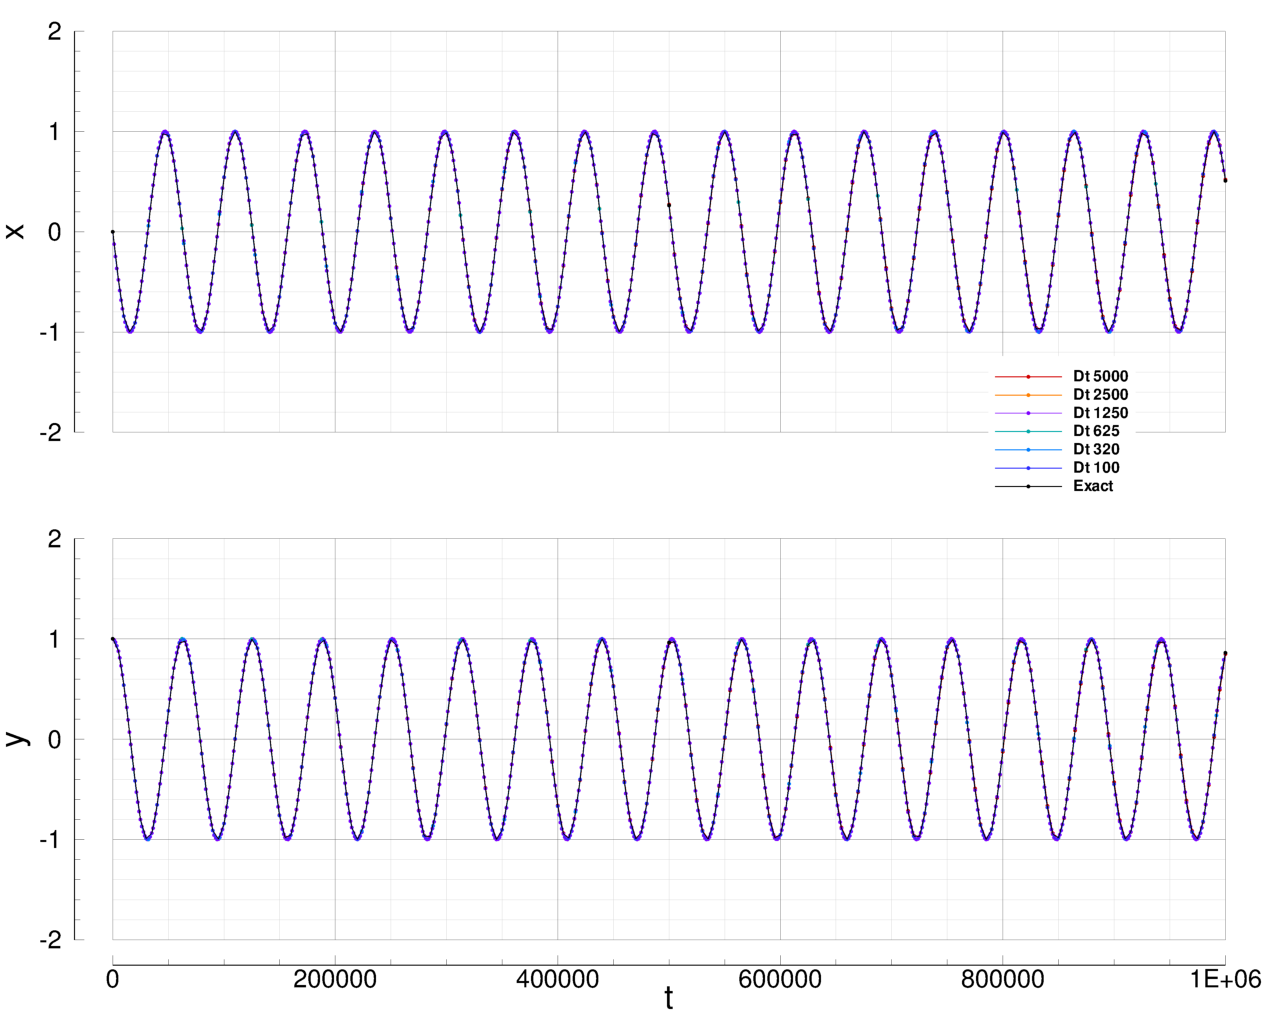
\includegraphics[width=0.70\textwidth]{errors-analysis/oscillation/error_analysis-oscillation-ls-runge-kutta-5.png}
  \caption{Oscillation equations solutions computed by means of low storage Runge-Kutta 5 stages solver}\label{fig:results-oscillation-ls-runge-kutta-5}
\end{figure}

\paragraph{TVD/SSP Runge-Kutta}

\begin{figure}[!ht]
  \centering
  \includegraphics[width=0.70\textwidth]{errors-analysis/oscillation/error_analysis-oscillation-tvd-runge-kutta-2.png}
  \caption{Oscillation equations solutions computed by means of TVD/SSP Runge-Kutta 2 stages solver}\label{fig:results-oscillation-tvd-runge-kutta-2}
\end{figure}

\begin{figure}[!ht]
  \centering
  \includegraphics[width=0.70\textwidth]{errors-analysis/oscillation/error_analysis-oscillation-tvd-runge-kutta-3.png}
  \caption{Oscillation equations solutions computed by means of TVD/SSP Runge-Kutta 3 stages solver}\label{fig:results-oscillation-tvd-runge-kutta-3}
\end{figure}

\begin{figure}[!ht]
  \centering
  \includegraphics[width=0.70\textwidth]{errors-analysis/oscillation/error_analysis-oscillation-tvd-runge-kutta-5.png}
  \caption{Oscillation equations solutions computed by means of TVD/SSP Runge-Kutta 5 stages solver}\label{fig:results-oscillation-tvd-runge-kutta-5}
\end{figure}

\clearpage

\section{Ongoing Development Activities}\label{sec:ongoing}

\section{Concluding Remarks and Perspectives}\label{sec:conclusions}

\bibliographystyle{mycpc2}
\bibliography{Reference}

\end{document}
